%%%%%%%%%%%%%%%%%%%%%%%%%%%%%%%%%%%%%%%%%%%%%%%%%%%%%%%%%%%%%%%%%%%%%%%%%%%%%%%%
\chapter{Leistungsanalyse}
\label{sct:benchmarks}
%%%%%%%%%%%%%%%%%%%%%%%%%%%%%%%%%%%%%%%%%%%%%%%%%%%%%%%%%%%%%%%%%%%%%%%%%%%%%%%%

%%%%%%%%%%%%%%%%%%%%%%%%%%%%%%%%%%%%%%%%%%%%%%%%%%%%%%%%%%%%%%%%%%%%%%%%%%%%%%%%
\section{Testsystem}
\label{sct:taurus}
%%%%%%%%%%%%%%%%%%%%%%%%%%%%%%%%%%%%%%%%%%%%%%%%%%%%%%%%%%%%%%%%%%%%%%%%%%%%%%%%


Für die Skalierungstests wurde Taurus, einer der Hochleistungsrechner der TU-Dresden, benutzt.
Der Bau der ersten Phase von Taurus war 2013 abgeschlossen\cite{taurusnutzerschulung}.
Zum Zeitpunkt der Nutzung (2015/2016) waren alle Knoten von Phase 1, vgl. \autoref{fig:taurusphase1} links, in die 2015 fertiggestellt\cite{heisehrsk2} Phase 2, siehe \autoref{fig:taurusphase1} rechts, integriert \cite{doctudtaurushardware}. Gerechnet wurde je nach Verfügbarkeit auf Phase 1 oder 2 von Taurus, vgl. Tabelle~\ref{tbl:island2}.

\begin{figure}[H]
	\centering
	\begin{minipage}{0.5\linewidth}
		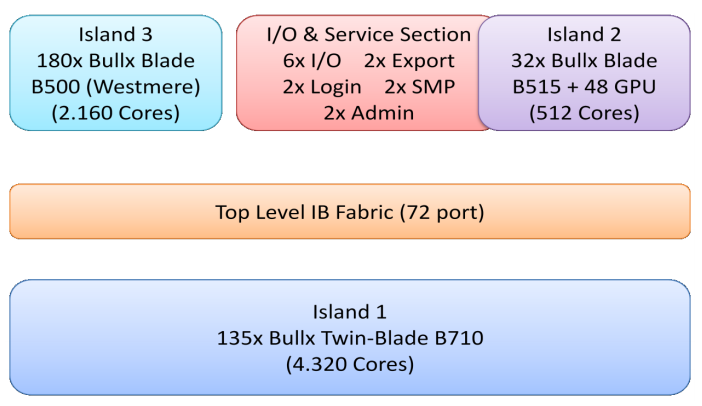
\includegraphics[width=\linewidth]{taurusphase1}
	\end{minipage}\begin{minipage}{0.5\linewidth}
		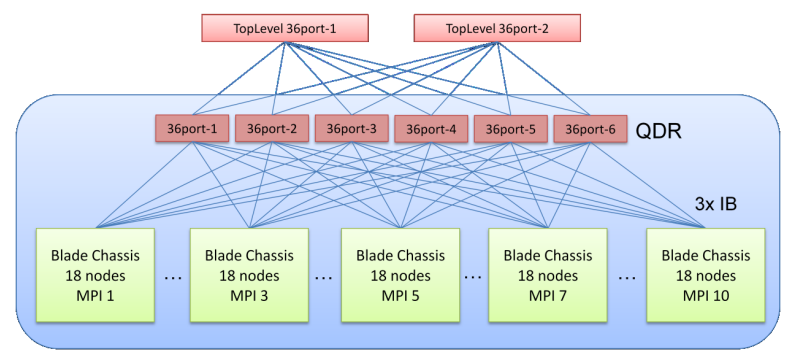
\includegraphics[width=\linewidth]{taurusphase1island1interconnects}
	\end{minipage}
	\caption{\textbf{Links:} Übersicht Taurus Phase 1. \textbf{Rechts:} Schema der Topologie von Insel 2, auf der ausschließlich gerechnet wurde. Die Bilder wurden übernommen aus Ref.\cite{taurusnutzerschulung}}
	\label{fig:taurusphase1}
\end{figure}

\begin{table}[H]
	\begin{tabularx}{0.9\linewidth}{r|Y|Y}
		& \textbf{Phase 1} & \textbf{Phase 2} \\
		\hline
		Knoten          & 44 & 64 \\
		Hostnamen       & taurusi2[001-044] & taurusi2[045-108] \\
		Prozessor       & 2x Intel Xeon CPU E5-2450 (8 Kerne) zu je \SI{2.10}{\giga\hertz}, MultiThreading deaktiviert, AVX, 2x 268.8\,GSPFLOPS \cite{2400flops}
						& 2x Intel(R) Xeon(R) CPU E5-2680 v3 (12 Kerne) zu je \SI{2.50}{\giga\hertz}, MultiThreading deaktiviert, AVX2 insbesondere FMA3\cite{ark2680v3}, 2x 480\,GSPFLOPS\cite{e5microway} \\
		GPU 			& 2x NVIDIA Tesla K20X & 4x NVIDIA Tesla K80 \\
		Arbeitsspeicher & \SI{32}{\gibi\byte} & \SI{64}{\gibi\byte} \\
		Festplatte      & \SI{128}{\gibi\byte} SSD & \SI{128}{\gibi\byte} SSD
	\end{tabularx}
	\caption{Zusammensetzung Insel 2 von Taurus\cite{doctudtaurussystem}}
	\label{tbl:island2}
\end{table}

\begin{table}[H]
	\begin{tabular}{r|c|c}
	& \textbf{K20X} & \textbf{K80} \\
	\hline
	Chip       & GK110 & GK210 \\
	Takt       & \SI{0.732}{\giga\hertz} & \SI{0.560}{\giga\hertz} \\
	CUDA-Kerne & 2688 & 4992 \\
	Speicher   & \SI{6}{\gibi\byte}, GDDR5 384 Bit Busbreite
	           & $2\times\SI{12}{\gibi\byte}$, GDDR5 384 Bit Busbreite \\
    Bandbreite & \SI{250}{\giga\byte\per\second}
	           & $2\times\SI{240}{\giga\byte\per\second}$              \\
%	\begin{minipage}{2.5cm}\begin{flushright}Theoretische\\Spitzenleistung\end{flushright}\end{minipage} & 3935\,GSPFLOPS, 1312\,GDPFLOPS
%					& 5591\,GSPFLOPS, 1864\,GDPFLOPS \\
	Theoretische    & 3935\,GSPFLOPS & 5591\,GSPFLOPS \\
	Spitzenleistung & 1312\,GDPFLOPS & 1864\,GDPFLOPS
	\end{tabular}
	\caption{Spezifikationen der Kepler-Grafikkarten von Taurus\cite{nvidiakepler,k20anandtech}}
	\label{tbl:k20k80}
\end{table}

Zu den Spitzenleistungen in Tabelle~\ref{tbl:k20k80} sei angemerkt, dass jeder CUDA-Kern eine Operation einfacher Fließkommagenaugigkeit oder eine 32-Bit Integeroperation berechnen kann und dass auf drei CUDA-Kerne eine Doppelpräzisionseinheit kommt, wodurch sich die DFLOPS berechnen.
Die K80 hat außerdem einen Boost-Modus mit \SI{0.875}{\giga\hertz}, also einer Leistungssteigerung von $1.56$.

Für z.B. die Tesla K20X beträgt die Maximalleistung in der Berechnung von Fließkommazahlen einfacher Genauigkeit (Single Precision Floating Point Operations Per Second - SPFLOPS) im Verhältnis einer Multiplikation zu einer Addition:
\begin{align}
	\SI{0.732}{\giga\hertz} \cdot 2688\,\text{CUDA-Kerne} \cdot
	1\,\frac{ \text{FMA-Einheit} }{ \text{CUDA-Kern} } \cdot
	2\,\frac{ \text{SPFLO} }{ \text{FMA-Einheit} }
	= 3935\,\text{GSPFLOPS}
\end{align}

Für den z.B. den Xeon E5-2680 v3 Prozessor beträgt die Maximalleistung:
\begin{align}
	\SI{2.50}{\giga\hertz} \cdot
	12\,\text{Kerne} \left(
		1\,\frac{ \text{AVX ADD Einheit} }{ \text{Kern} } +
		1\,\frac{ \text{AVX MUL Einheit} }{ \text{Kern} }
	\right) \cdot
	8\,\frac{ \text{SPFLO} }{ \text{AVX Einheit} } \\
	= 480\,\text{GSPFLOPS}
\end{align}


%%%%%%%%%%%%%%%%%%%%%%%%%%%%%%%%%%%%%%%%%%%%%%%%%%%%%%%%%%%%%%%%%%%%%%%%%%%%%%%%
\section{Profiling}
%%%%%%%%%%%%%%%%%%%%%%%%%%%%%%%%%%%%%%%%%%%%%%%%%%%%%%%%%%%%%%%%%%%%%%%%%%%%%%%%

Profiling mit dem NVIDIA Visual Profiler ist auch mit Rootbeer möglich.
Dafür muss als ausführbare zu analysierende Datei jedoch \lstinline!java! mit den Argumenten zu der auszuführenden JAR-Datei angegeben werden:
\begin{lstlisting}[language=bash, caption={Erstellen der Profiling-Daten}, label={lst:nvprof}]
sbatch --time=00:30:00 --nodes=1 --partition=gpu2 --cpus-per-task=4 --gres='gpu:4' <<EOF
#!/bin/bash
nvprof --analysis-metrics --metrics all \
-o $HOME/scaromare/MontePi/profilingDataMultiGpuScala.nvp%p \
$(which java) -jar $HOME/scaromare/MontePi/singleNode/multiGpu/scala/MontePi.jar $((2*14351234510)) 2
EOF
\end{lstlisting}
Die so erzeugten Zeitmessungen in \lstinline!profilingDataMultiGpuScala.nvp! können mit \lstinline!nvvp! ausgewertet und visualisiert werden.

In \autoref{fig:apicalls} ist ein Programmlauf mit zwei Grafikkarten zu sehen.
In der originalen Rootbeerversion wurde für jede Grafikkarte erst ein \lstinline!cuCtxCreate! aufgerufen, welches sehr zeitaufwändig ist, dann der freie Grafikkartenspeicher der Grafikkarte abgerufen und zuletzt der Kontext wieder mit \lstinline!cuCtxDestroy! gelöscht, siehe auch Seite~\pageref{pg:cuCtxCreate} und \autoref{fig:apicalls} oben.
Dies wurde im eigenen Fork behoben, sodass nur noch ein Aufruf zu \lstinline!cuCtxCreate! für die Grafikkarte, die auch wirklich benutzt wird, notwendig ist, siehe \autoref{fig:apicalls} unten.
Die Gesamtlaufzeit im Beispiel wurde so von ca. \SI{8}{\second} auf \SI{5}{\second} reduziert.

\begin{figure}
	\begin{center}
		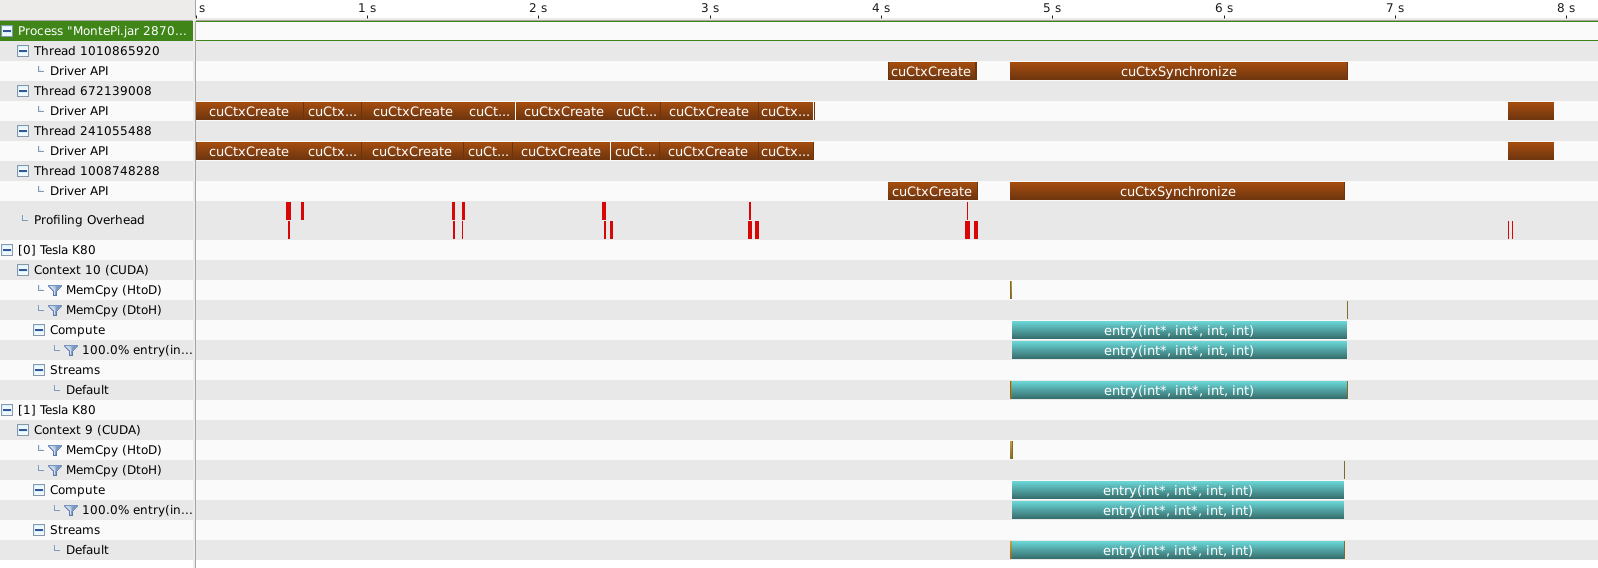
\includegraphics[width=\linewidth]{../MontePi/profiling/2of4-APICalls.png}\\
		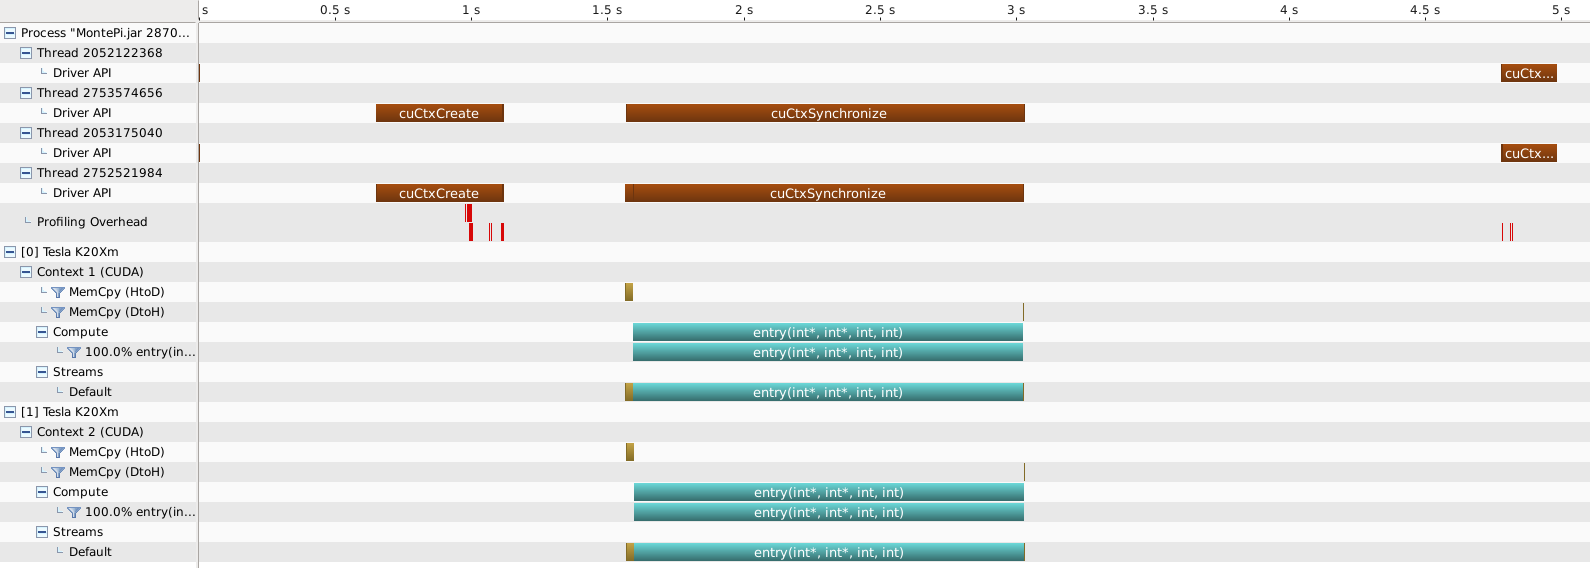
\includegraphics[width=\linewidth]{../MontePi/profiling/2of2-afterLoadDevicesPerformanceFix.png}
	\end{center}
	\caption{Profiling der CUDA-API-Aufrufe. \textbf{Oben:} Vor dem \lstinline!cuCtxCreate!-Fix im Rootbeerfork ausgeführt auf einem Tesla K80-Knoten. \textbf{Unten:} Nach dem Fix ausgeführt auf einem Tesla K20X-Knoten.}
	\label{fig:apicalls}
\end{figure}


%%%%%%%%%%%%%%%%%%%%%%%%%%%%%%%%%%%%%%%%%%%%%%%%%%%%%%%%%%%%%%%%%%%%%%%%%%%%%%%%
\section{Monte-Carlo-Simulation verschiedener Implementationen}
%%%%%%%%%%%%%%%%%%%%%%%%%%%%%%%%%%%%%%%%%%%%%%%%%%%%%%%%%%%%%%%%%%%%%%%%%%%%%%%%

In Abb.\ref{fig:montepiworkloadscaling} wurde die Ausführungszeit von Monte-Carlo-Simulationen implementiert mit verschiedenen Programmiersprachen über die Anzahl an Monte-Carlo-Iterationen gemessen.
Die Zeit wurde mit dem Linux \lstinline!time!-Befehl gemessen. Dieser Befehl gibt real-, user- und sys-Zeit aus; die real-Zeit wird für den Benchmark genutzt.

Jede Implementation hat eine gewisse Initialisierungszeit. Bei der C++-Version beträgt diese jedoch nur knapp \SI{70}{\milli\second}, während die reine Java-Version schon ca. \SI{220}{\milli\second} benötigt.
Die Nutzung von Scala erhöht dies auf \SI{250}{\milli\second} und die Nutzung von Rootbeer führt eine weitere Initialisierungszeit von \SI{2}{\second} ein, sodass für wenig Iterationen die Rootbeerversion bis zu 20x langsamer sind als die Hostprozessorversionen.
Die Rootbeerinitialisierungszeit beinhaltet das Entpacken der benötigten Binärdateien, das Erstellen des CUDA-Kontextes und den Transfer der Daten zwischen GPU und Host.
Die hier nicht gemessene Spark-Implementierung benötigte in Einzeltests noch mehr Zeit für die Initialisierung.

Erst für 10 Milliarden Iterationen beginnt die Initialisierungszeit der Rootbeer-Implementierungen im Vergleich zur Rechenzeit vernachlässigbar zu werden, sodass ab da die Lastenskalierung ein lineares Verhalten annimmt.
Bei der C++-Version ist dies indes schon bei ca. 100 Millionen Iterationen der Fall.
\begin{figure}
	\centering
	\begin{minipage}{0.7\linewidth}
		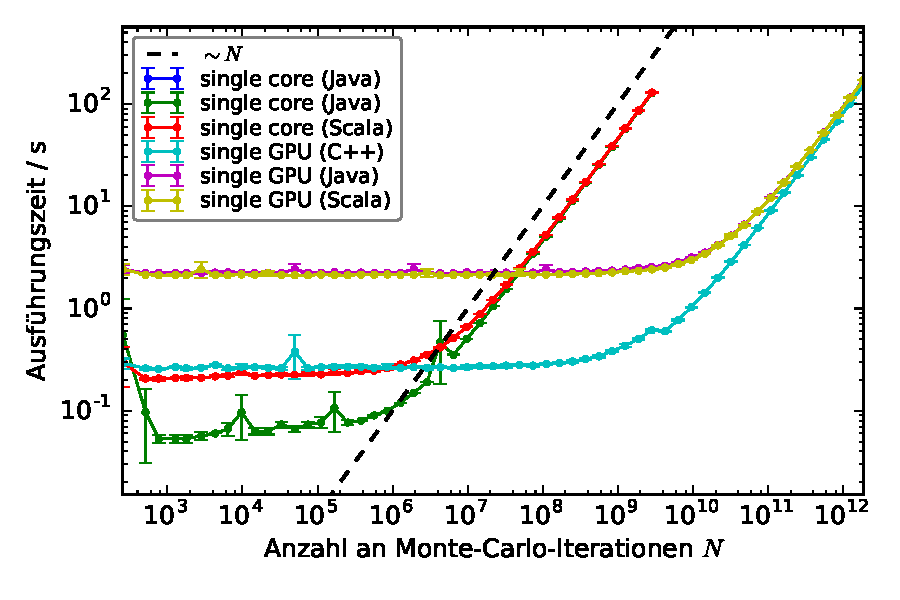
\includegraphics[width=\linewidth]{../MontePi/benchmark/benchmarks-workload-scaling.pdf}
	\end{minipage}
	\caption{Benötigte Ausführungszeit der Monte-Carlo Pi-Berechnung in Abhängigkeit von der Anzahl an Iterationen. Getestet auf Taurusknoten \lstinline!taurusi2095! und \lstinline!taurusi2105!, also auf Tesla K80-Knoten, siehe \autoref{sct:taurus}}
	\label{fig:montepiworkloadscaling}
\end{figure}

Weiterhin ist aus dem Plot abzulesen, dass für große Lasten wie z.B. für drei Milliarden Iterationen die Versionen, die von Grafikarten Gebrauch machen, um einen Faktor $50$ (Scala) bis $210$ (C++) schneller sind als die Implementierungen, die auf einem Prozessor-Kern ausgeführt werden.
Die theoretische Maximalleistung eines Kerns auf dem Intel Xeon E5-2680v3-Knoten beträgt $40\,\text{GSPFLOPS}$.
Das heißt man würde einen Speedup von ca. $140\,\text{GSPFLOPS}$ erwarten.
Dass der Speedup höher ist liegt wahrscheinlich daran, dass Java keinen oder nur schlecht optimierten Gebrauch von AVX für die Monte-Carlo-Berechnung macht.

\begin{figure}[H]
	\centering
	\begin{minipage}{0.7\linewidth}
		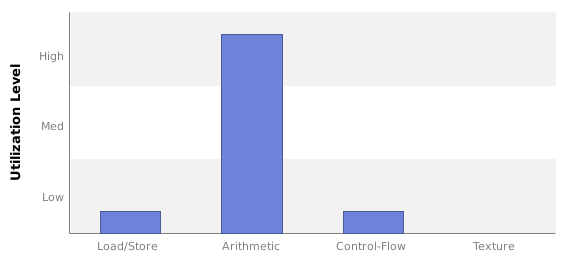
\includegraphics[width=\linewidth]{../presentation/kernel-utilization}
	\end{minipage}
	\caption{Auswertung der Kernel-Utilisierung mit dem NVIDIA Visual Profiler des mit Rootbeer beschleunigten Monte-Carlo-Algorithmus.}
	\label{fig:utilization}
\end{figure}


Die Auswertung der Utilisierung in \autoref{fig:utilization} zeigt, dass der Algorithmus die arithmetischen Einheiten fast voll auslastet.
Es ist also noch Spielraum für Algorithmen die weniger rechenlastig sind und mehr Speicherzugriffe haben.
Im Allgemeinen wird es sich aber nicht lohnen Algorithmen zu parallelisieren, die gleich viel Speicherzugriffe wie Berechnungen haben.
Gut geeignet sind Algorithmen, bei denen die Anzahl an Berechnungen mit dem Quadrat der Anzahl an Speicherzugriffen oder noch schneller steigt.


%%%%%%%%%%%%%%%%%%%%%%%%%%%%%%%%%%%%%%%%%%%%%%%%%%%%%%%%%%%%%%%%%%%%%%%%%%%%%%%%
\section{Monte-Carlo-Simulation mit Spark und Rootbeer}
%%%%%%%%%%%%%%%%%%%%%%%%%%%%%%%%%%%%%%%%%%%%%%%%%%%%%%%%%%%%%%%%%%%%%%%%%%%%%%%%

In Abbildung~\ref{fig:montepiweakscaling} ist die Laufzeit über die Anzahl an Grafikkarten dargestellt. jeder Knoten hat zwei Tesla K20X-Grafikkarten.
Die Anzahl an Iterationen wurde proportional zu der Anzahl an Grafikkarten erhöht, sodass jede Grafikkarte immer gleich viel Arbeit hat.
Man erwartet also, dass die Ausführungszeit unabhängig von der Anzahl an Grafikkarten konstant bleibt, wie es auch der Fall ist.

Ab 16,17,18, in einem Einzelfall auch 19 Grafikkarten steigen jedoch die Laufzeiten plötzlich um ca. \SI{1}{\second} an, sodass der Speedup sich vom idealen Speedup entfernt, das heißt die parallele Effizienz nimmt ab.
Die genaue Ursache hierfür wurde nicht gefunden.
Mögliche Ursachen könnte Spark, Straggler, das Verbindungsnetzwerk oder vielleicht auch Rootbeer sein.
Interessant wäre auch eine Wiederholung des Tests auf einem K80-System und jeweils mit mehr als 32 Grafikkarten, um eine weitere Erhöhung der Laufzeit bei Vielfachen von 16 Grafikkarten auszuschließen.
Aus Rechenzeitgründen war dies jedoch zum aktuellen Zeitpunkt nicht mehr möglich.

\begin{figure}[H]
	\centering
	\begin{minipage}{0.5\linewidth}
		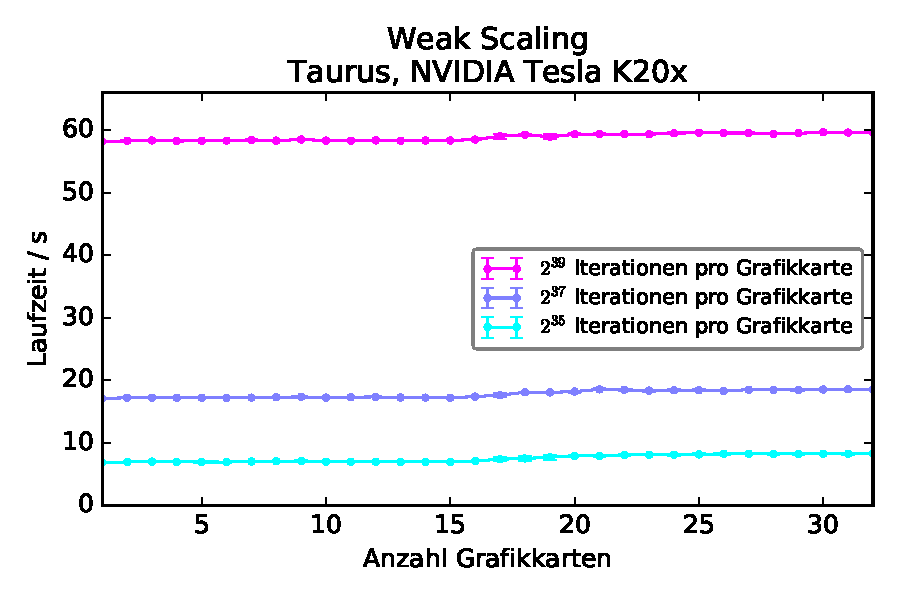
\includegraphics[width=\linewidth]{../MontePi/benchmark/weak-scaling-time-gpu.pdf}
	\end{minipage}\begin{minipage}{0.5\linewidth}
		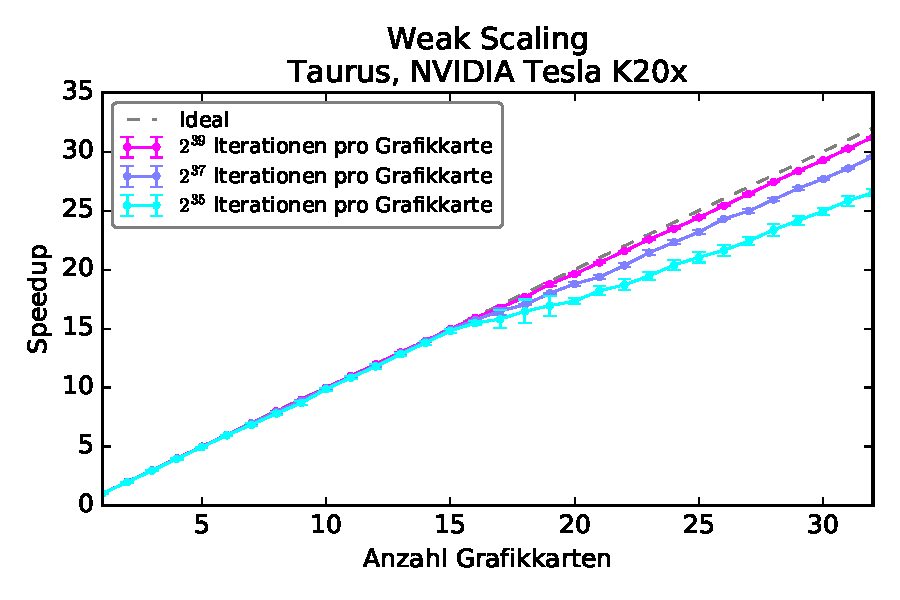
\includegraphics[width=\linewidth]{../MontePi/benchmark/weak-scaling-speedup-gpu.pdf}
	\end{minipage}
    \centerline{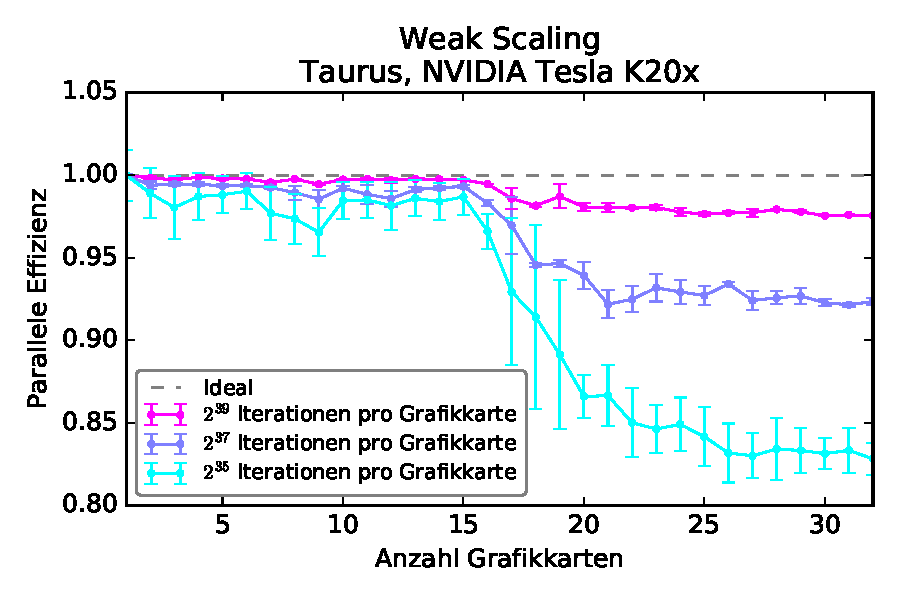
\includegraphics[width=0.5\linewidth]{../MontePi/benchmark/weak-scaling-efficiency-gpu.pdf}}
	\caption{Benötigte Ausführungszeit der Monte-Carlo Pi-Berechnung in Abhängigkeit von der Anzahl an Grafikkarten gemessen auf Tesla K20X-Knoten. \textbf{Links:} Absolute Ausführungszeiten der Spark-Map-Funktion. \textbf{Rechts:} Speedup bezüglich der Laufzeit mit einer Grafikkarte. \textbf{Unten:} Parallele Effizienz}
	\label{fig:montepiweakscaling}
\end{figure}

Weiterhin wurden die Benchmarks wiederholt für vier fixierte Totalproblemgrößen, sodass die Arbeit pro Grafikkarte mit Erhöhung der Parallelisierung abnimmt.
Wie man in \autoref{fig:montepistrongscaling} sieht nimmt also mit Erhöhung der Grafikkarten die Laufzeit so lange proportional ab, bis der Großteil der benötigten Zeit nur noch aus der seriellen Initialisierungszeit besteht und sich somit der wirklich erreichte Speedup sättigt, vergleiche auch mit dem Amdahlschen Gesetz.

Für $2^37=137\cdot 10^9$ Gesamtiterationen ist der Speedup bei ungefähr vier gesättigt.
Es ist also nicht sinnvoll dieses dieses Problem mit signifikant mehr als vier Grafikkarten zu parallelisieren.
Wie aus \autoref{fig:montepiworkloadscaling} entnehmbar würde die CPU-Version ungefähr \SI{500}{\second} benötigen.
Es ist also erst bei sehr großen Problemen, die auf dem Host mehr als eine Minute benötigen würden, überhaupt sinnvoll Grafikkarten einzusetzen.

Wenn auf dem Host AVX und alle Kerne benutzt werden, dann muss das Problem noch größer sein, damit sich Grafikkarten lohnen.
Wenn die Probleme aber genügend groß sind, dann rentieren sich Grafikkartenbeschleuniger sehr.
Bei ungefähr vergleichbaren Prozessoren zu Grafikkarten und beiderseits sehr gut optimierten Programmen ist, wie in \autoref{tbl:k20k80} an den theoretischen Peak-FLOPS zu sehen, ein 10-facher Geschwindigkeitsgewinn realistisch.
Dies gilt jedoch nur für einfache Genauigkeit.
Für Fließkommaberechnungen doppelter Genauigkeit sind Grafikkarten je nach Modell ungeeignet.

\begin{figure}[H]
	\centering
	\begin{minipage}{0.5\linewidth}
		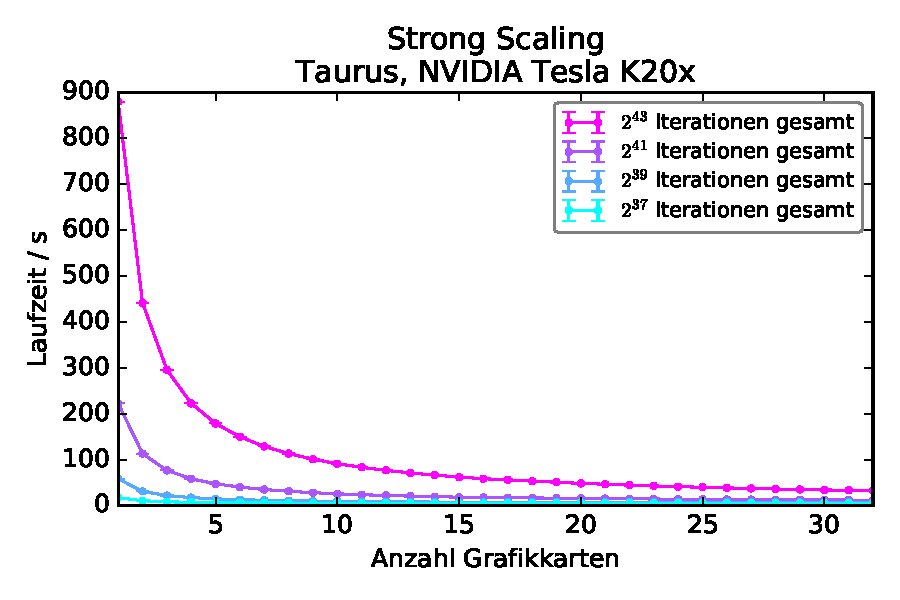
\includegraphics[width=\linewidth]{../MontePi/benchmark/strong-scaling-time-gpu.pdf}
	\end{minipage}\begin{minipage}{0.5\linewidth}
		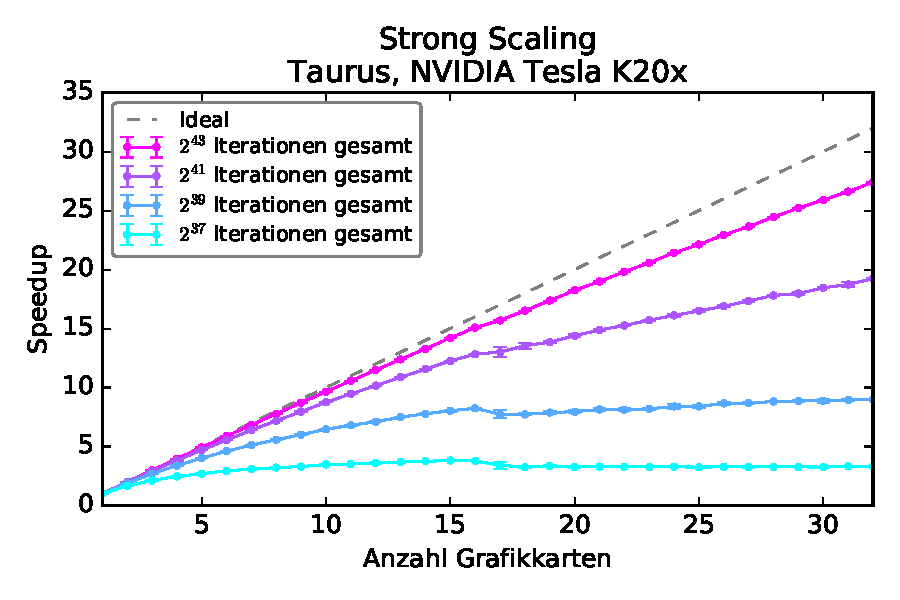
\includegraphics[width=\linewidth]{../MontePi/benchmark/strong-scaling-speedup-gpu.pdf}
	\end{minipage}
    \centerline{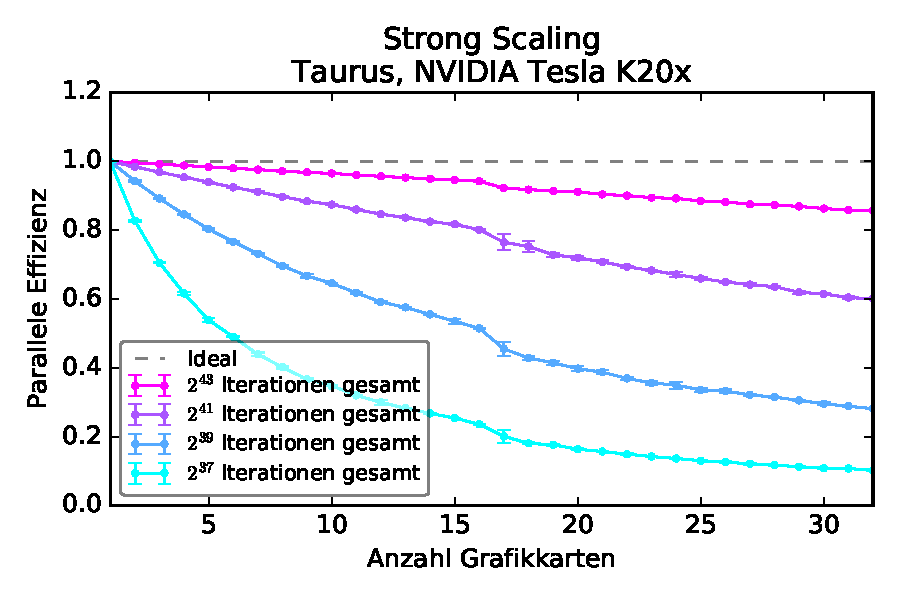
\includegraphics[width=0.5\linewidth]{../MontePi/benchmark/strong-scaling-efficiency-gpu.pdf}}
	\caption{Benötigte Ausführungszeit der Monte-Carlo Pi-Berechnung in Abhängigkeit von der Anzahl an Grafikkarten gemessen auf Tesla K20X-Knoten. \textbf{Links:} Absolute Ausführungszeiten der Spark-Map-Funktion. \textbf{Rechts:} Speedup bezüglich der Laufzeit mit einer Grafikkarte. \textbf{Unten:} Parallele Effizienz}
	\label{fig:montepistrongscaling}
\end{figure}
